\chapter{DESTECS Summer School models} \label{chap:summerschoolmodels}

\section{Introduction}\label{chap:summerschoolintro}
In July 2012 the DESTECS project hosted a summer school for
postgraduate level students and practitioners, which included
multi-day projects in groups.  Five groups in total were set the
assignment of developing their own line-following robots, including
setting appropriate design priorities and testing out different
possible designs to achieve the optimum result.  We include these
models here, as they provide a good demonstration of how DESTECS can
facilitate the exploration of the design space.  These models are
provided as-is, showing the real work of first-time DESTECS users
working on a time-limited project, and should be viewed as such. Photos of each group, along with their designs, are shown in Figure~\ref{fig:groupphotos}.

Each group had the same brief: to develop a line-following robot model
as described in Chapter \ref{chap:lineFollowingRobot}.  Groups aimed
to create the `best' performing robot, where performance was measured
by total time taken to follow a given set of lines (not known in
advance) and how accurately the robot measured these lines.  Models
were required to measure the time taken and the distance of the line
for this reason.  It is assumed that the robot has a fixed starting
position which begins with a predictable pattern on the ground before
the line begins.

As described briefly in Chapter \ref{chap:lineFollowingRobot}, there
are several design aspects to consider:
\begin{itemize}
\item There was no limit on the number of sensors that could be added,
  and there was considerable possibility for groups to experiment with
  this.  Whilst it is possible to design a robot with only one sensor
  that would fulfil the requirements of the exercise, adding more
  sensors may allow the robot to plot a more accurate course.
\item Groups were free to change the position of the sensors as they
  saw fit.  A particular problem is posed by the difficulty of
  detecting sharp, acute angles, resulting in the line doubling
  sharply back on itself.  Some designs of robot will find these
  scenarios difficult to detect and will lose track of the line's
  location.  This can be made easier or more difficult by placing
  sensors further forward, further back, wider apart or closer
  together, and several groups did opt to experiment with alternative
  layouts to resolve the difficulty.
\item The motors that power the wheels for this particular robot can
  accept different voltages, which result in varying speeds being
  delivered to the wheels.  Groups can decide whether to implement
  higher speeds if they are confident of the line's course.  They can
  also decide how to effect a turn.  It is possible to turn with both
  wheels still moving forward (at different speeds); this approach
  prioritises speed.  Alternatively, it's also possible to halt one
  wheel or even reverse it in order to effect a turn; this approach
  minimises the distance travelled as the robot corners.
\end{itemize}

We present here the models that were created as they exhibit quite
different design choices.  Note that some library class files were
provided to ensure that all groups had the same basic environment in
which to operate and to produce a 3D simulation of the finished model;
these take the form of some classes in the DE model and some blocks in
the CT model.  In particular, all the CT models include a block
\texttt{RobotPhysics}, which incorporates blocks \texttt{LeftWheel}
and \texttt{RightWheel}, powered by blocks \texttt{LeftMotor} and
\texttt{RightMotor}.  Each wheel/motor combination also links to an
encoder (\texttt{encoderLeft} and \texttt{encoderRight}).  Outputs
from this block include data on the robot's current position and
angle, and the position of each wheel.  Inputs arrive from outside and
are delivered to the separate motors.

All groups were required to monitor rotations of the wheels for their
robot.  This is accomplished using a sensor that detects light and dark
which is mounted facing each wheel; it's assumed that the wheels of
the robot are marked with light and dark stripes that can be counted
as they move past the sensor.

Finally, the groups were given an initial set of shared design
parameters to use in their contract, including: two \keyw{real}
parameters for controlling the position of the sensors longitudinally
and laterally; one \keyw{real} for setting the encoder resolution; one
\keyw{real} for setting the initial angle or orientation of the robot;
and finally one \keyw{array} which contains the initial starting
co-ordinates (in the format x,y).  Groups could decide whether to
employ these or not; some groups opted not to and removed them from
the contracts, whilst others did not use all of the parameters but
left them in the contract for future development purposes.

\subsection{Usage}
We do not provide individual suggestions for each of these models as
their outward design parameters are very similar.  One good starting
point is to run a simulation for each robot, try out different line
patterns, and identify an optimal design out of the designs presented.
Each robot will handle different types of corners or curves
differently, and some have optimisations that allow them to move
faster over straight sections, or which allow them to turn more
quickly on a sharper corner.  Other robots prioritise an accurate
route over a speedy one.

Different groups chose to employ different numbers of sensors, and to
vary the positioning.  We recommend executing simulations with the
robots to see how different sensors may be employed, and effect that
it has on overall accuracy and speed.  The groups used the following
designs:
\begin{itemize}
\item \textbf{Group 1} used two sensors, placed symmetrically on the
  left and right.  Their model prioritises speed when turning.
\item \textbf{Group 2} used four sensors, two placed symmetrically
  (left and right) at the front of the robot, and two more also placed
  symmetrically towards the rear of the robot.  Group 2 also decided
  to vary the speed of the robot, so that on straight sections of
  track the robot moves more quickly, and also executes tight corners
  as fast as possible (the four-sensor design helps with this).
\item \textbf{Group 3} used three line sensors placed in a row, with
  the central sensor placed slightly further back than the left and
  right sensors.  Their model minimises distance taken to execute a
  turn by reversing one wheel.
\item \textbf{Group 4} also used three sensors, placed in a row.  They
  aimed to keep the central sensor directly over the line, so the
  extra middle sensor helps to improve course accuracy.
\item \textbf{Group 5} used two sensors, placed symmetrically on the
  left and right.  Their model minimises distance taken to execute
  turns.
\end{itemize}

The models generally use shared design parameters to control the
longitudinal and lateral positioning of the two sensors.  Another
worthwhile experiment therefore is to change the values of these
parameters to change the sensor position, and see how this affects
performance of the robot (distance travelled and time taken are
recorded by each model, so performance with different settings can be
compared).  Drastic changes to the position of the sensors may even
cause a robot's line-following algorithm to break, as assumptions made
by the algorithm about sensor location no longer hold true.  The
initial values of the parameters (for groups that use them) can be set
when running the model by opening the Debug window of the DESTECS tool
before running the co-simulation.

\newcommand{\picsize}{0.38\textwidth}
\begin{figure}[p]
\centering
\subfigure[Group 1]{\label{fig:group1}
  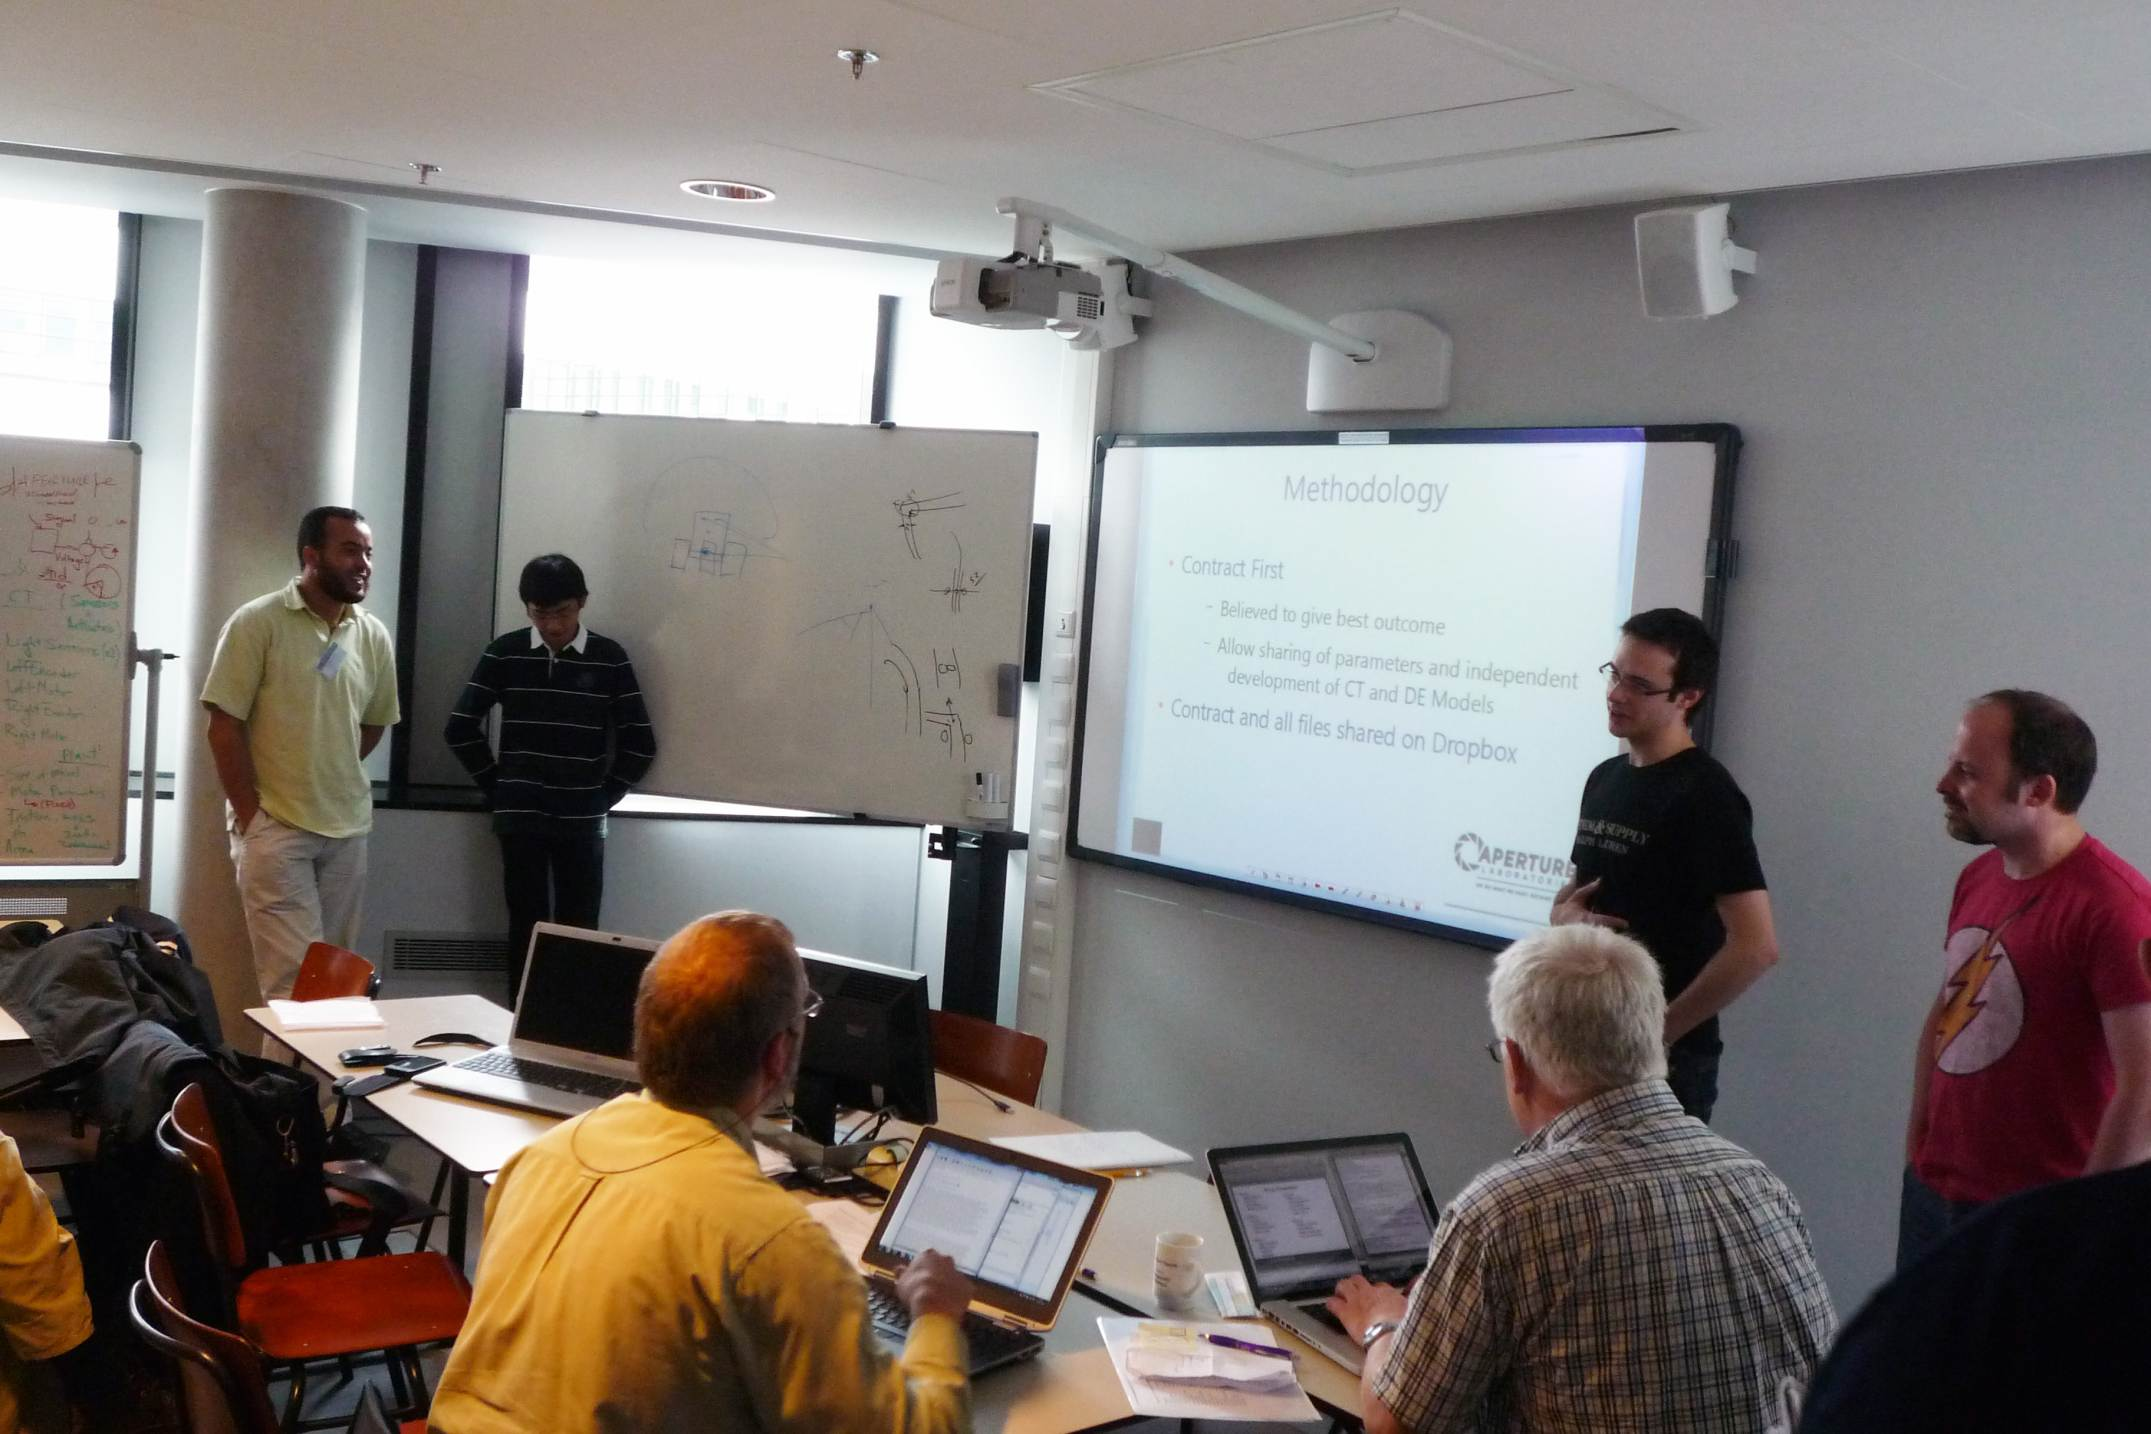
\includegraphics[width=\picsize]{summerSchoolModels/Group1} \quad
  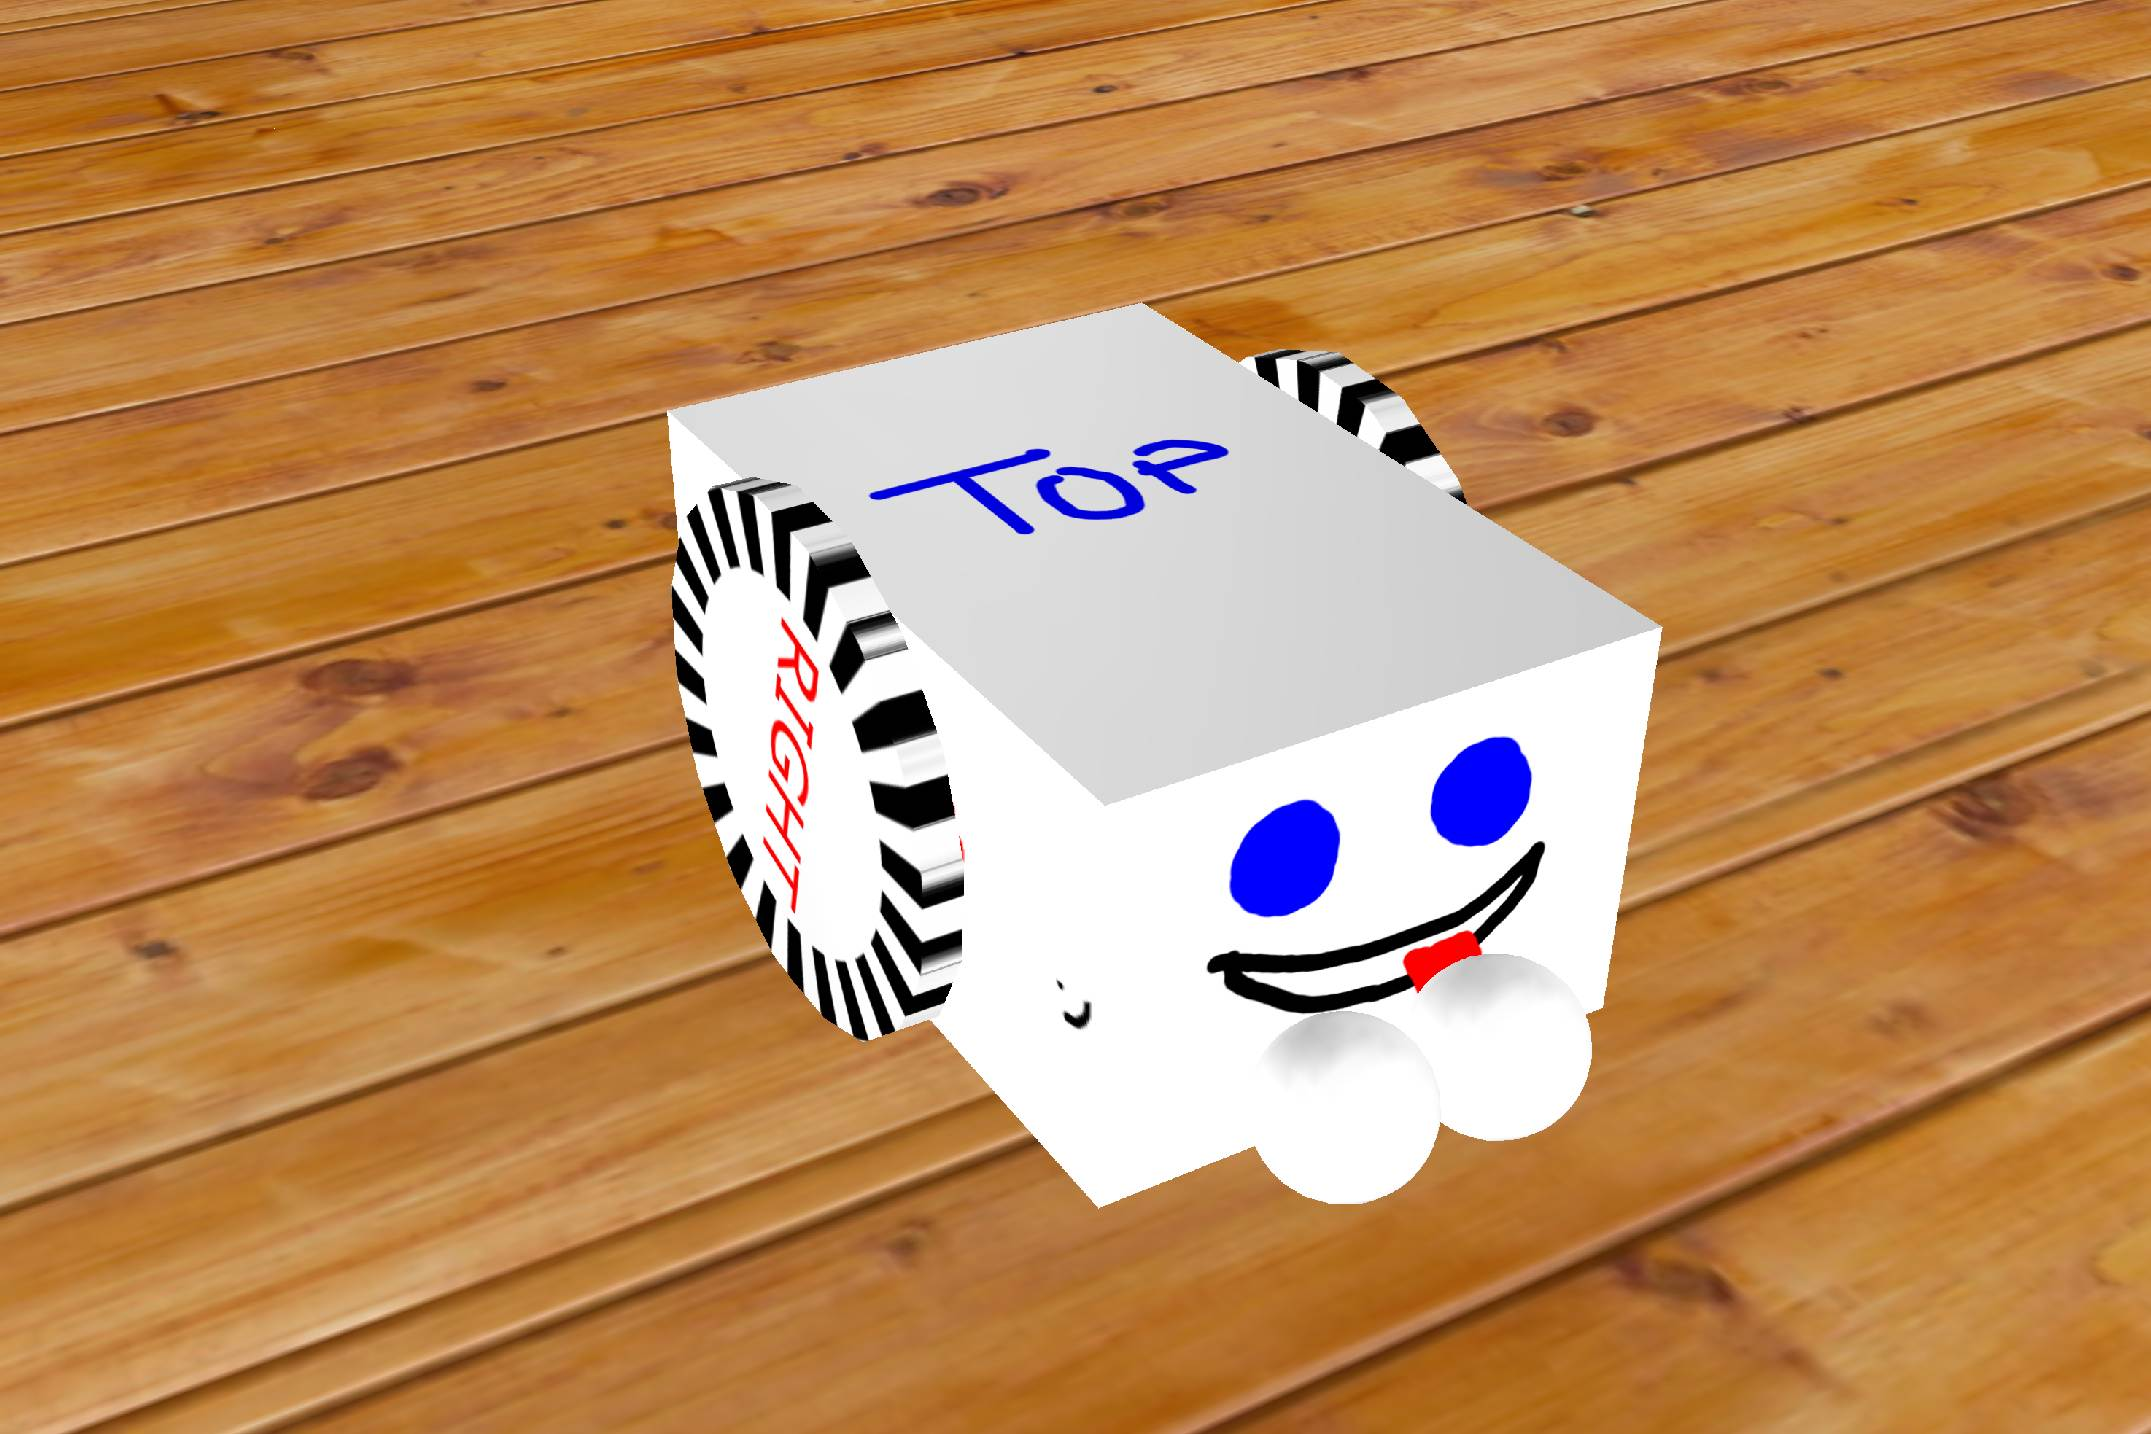
\includegraphics[width=\picsize]{summerSchoolModels/Group1robot}
} \\
\subfigure[Group 2]{\label{fig:group2}
  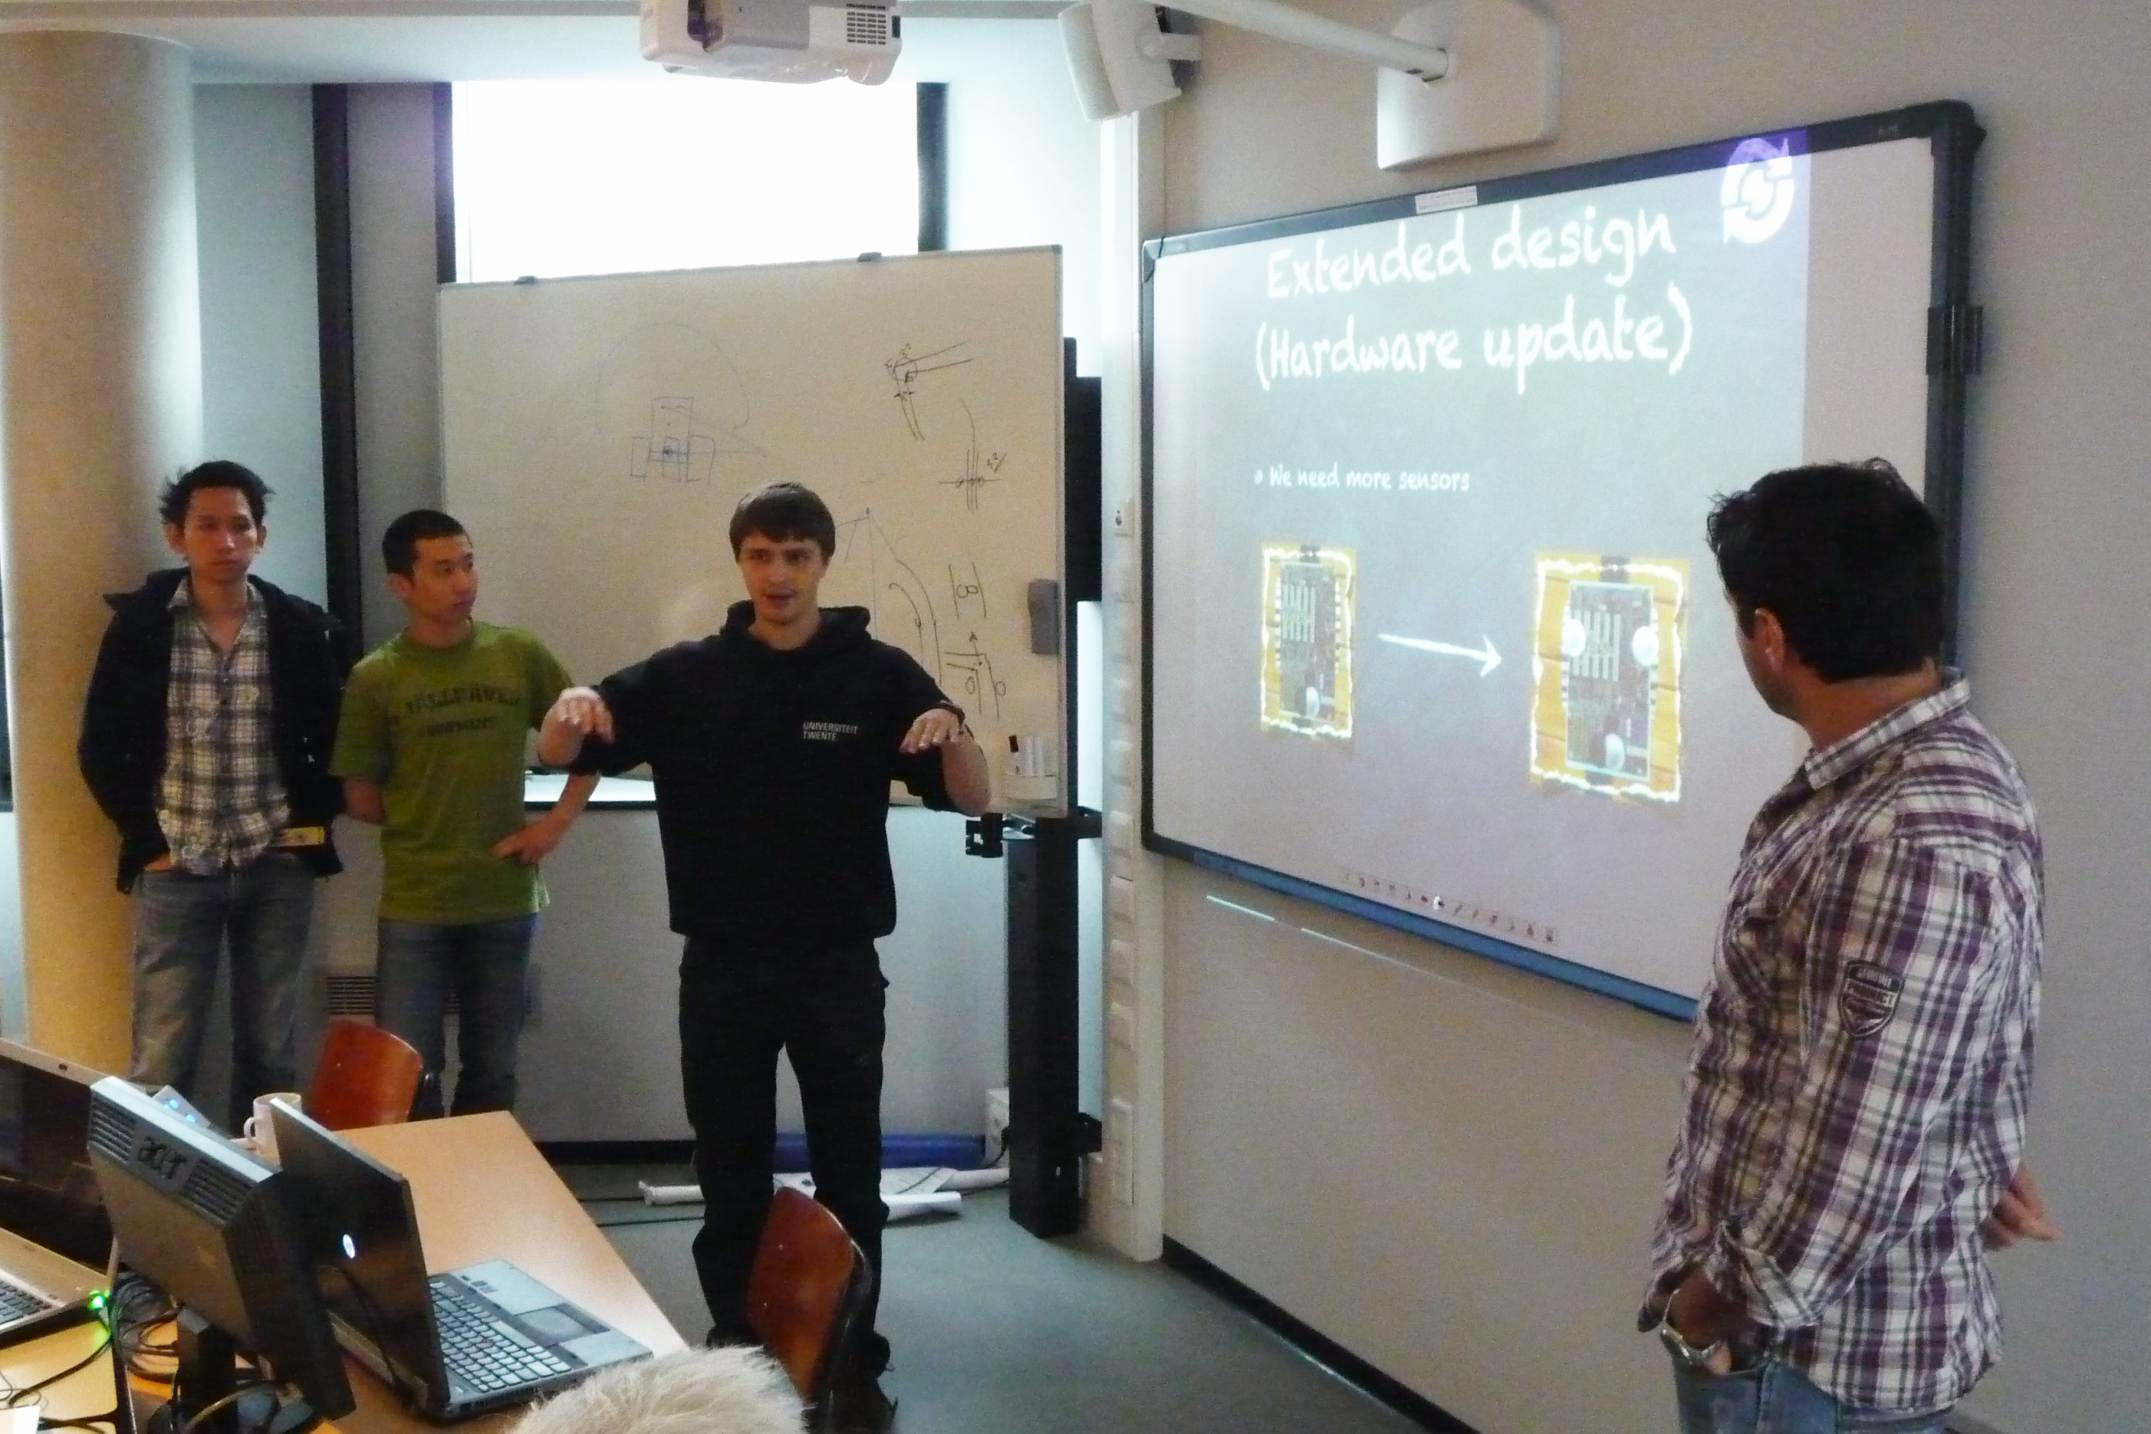
\includegraphics[width=\picsize]{summerSchoolModels/Group2} \quad
  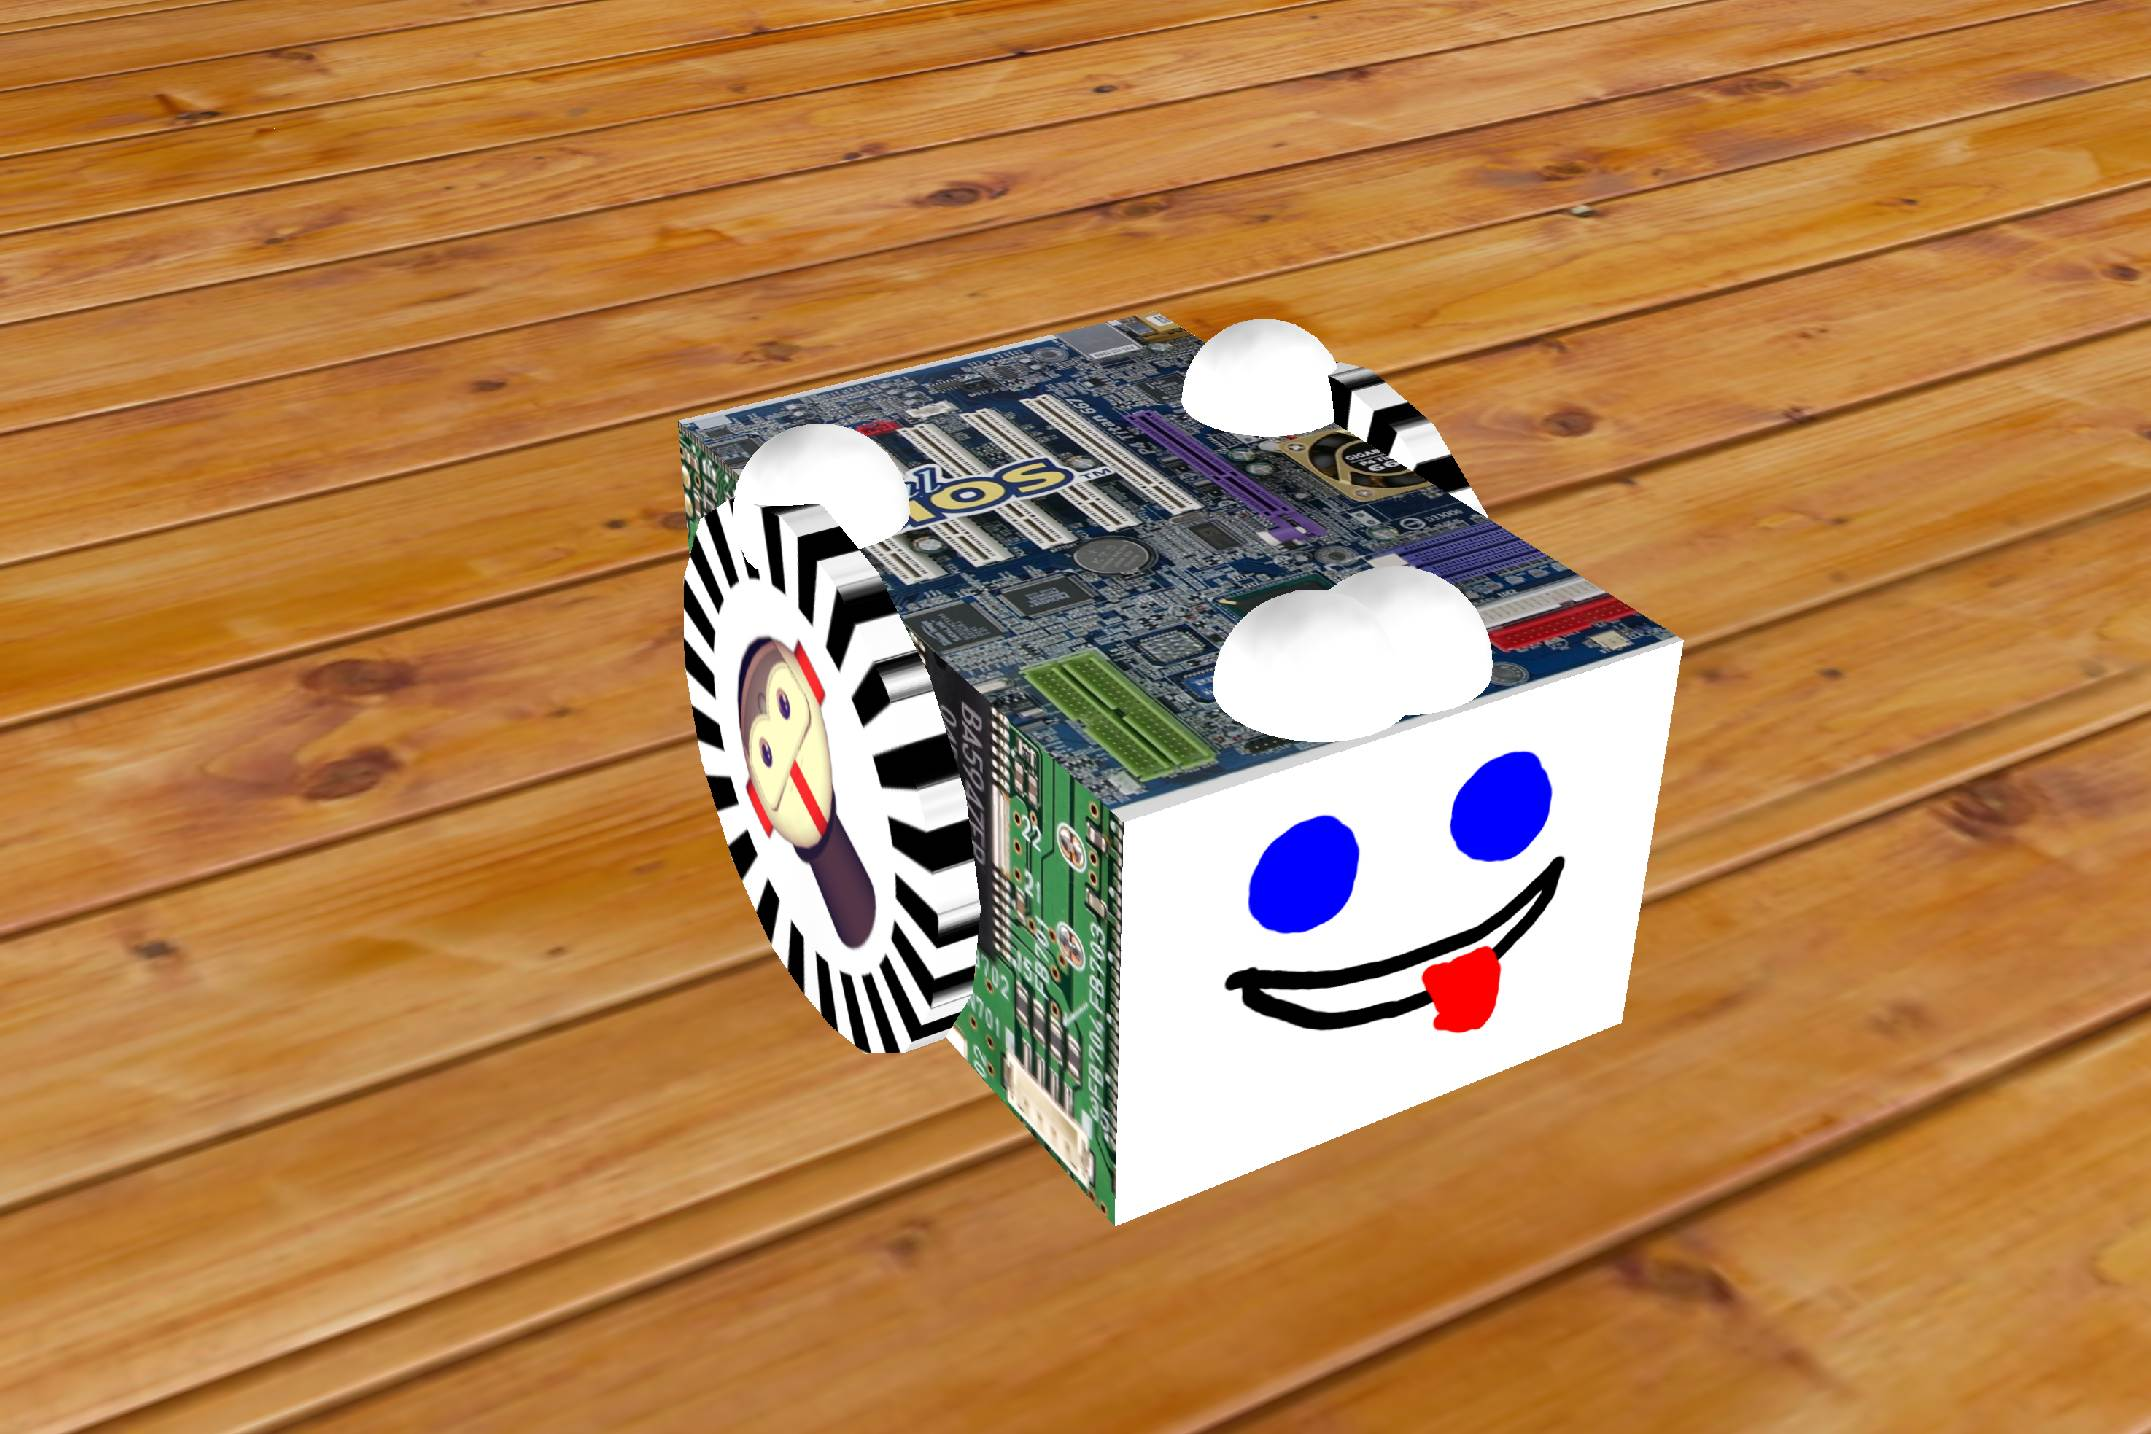
\includegraphics[width=\picsize]{summerSchoolModels/Group2robot}
} \\
\subfigure[Group 3]{\label{fig:group3}
  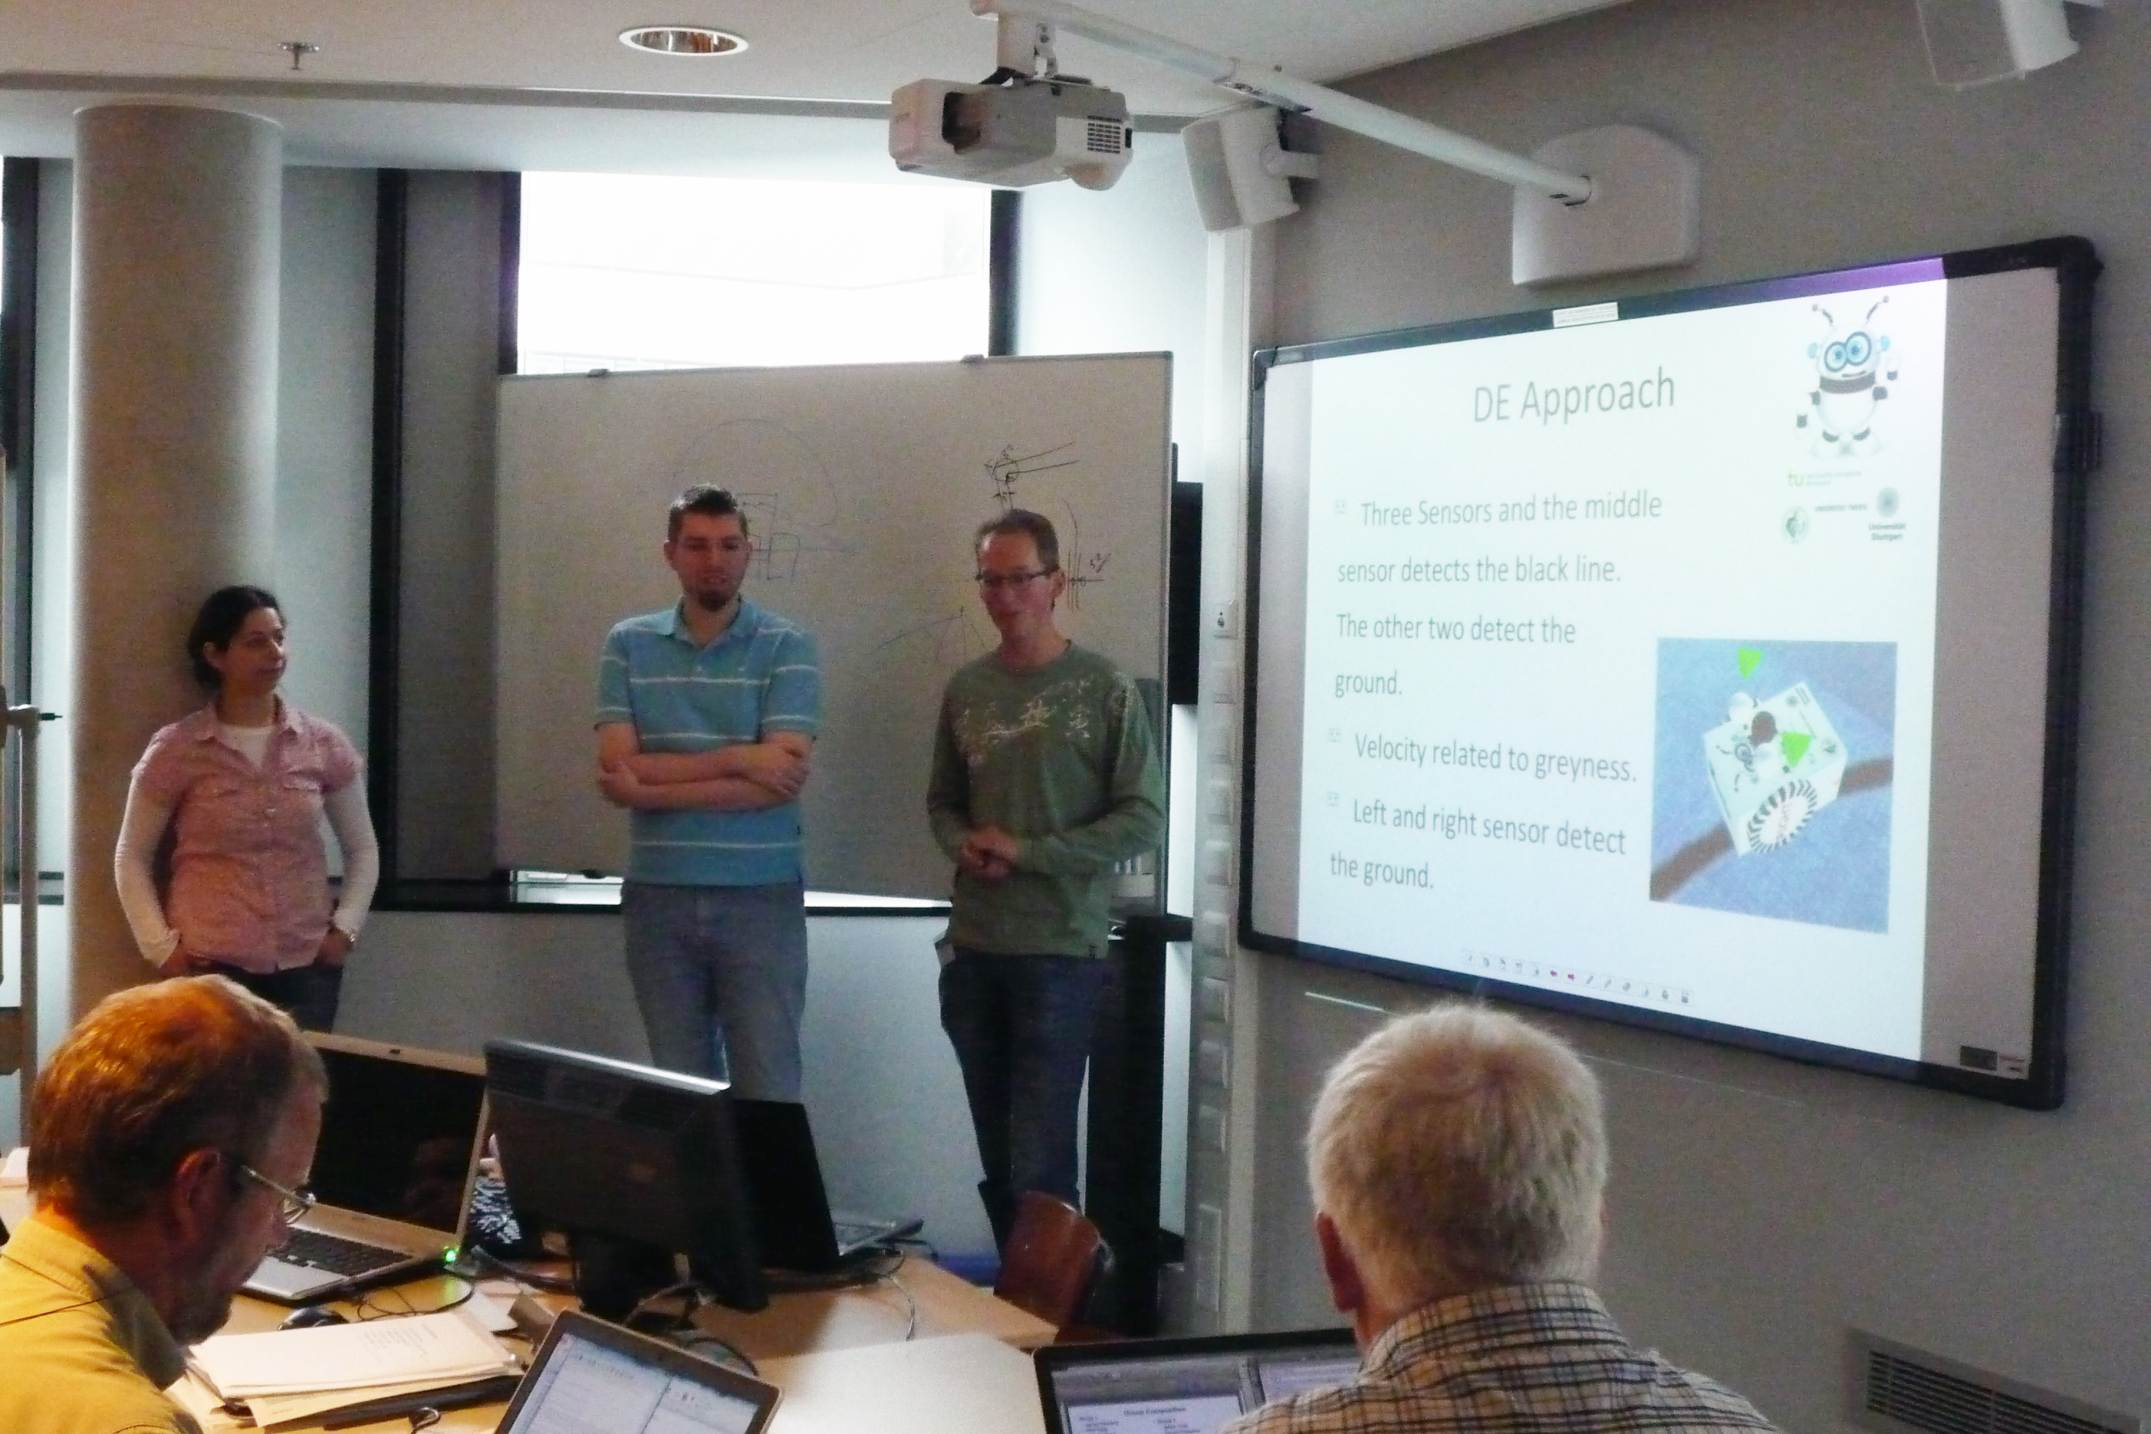
\includegraphics[width=\picsize]{summerSchoolModels/Group3} \quad
  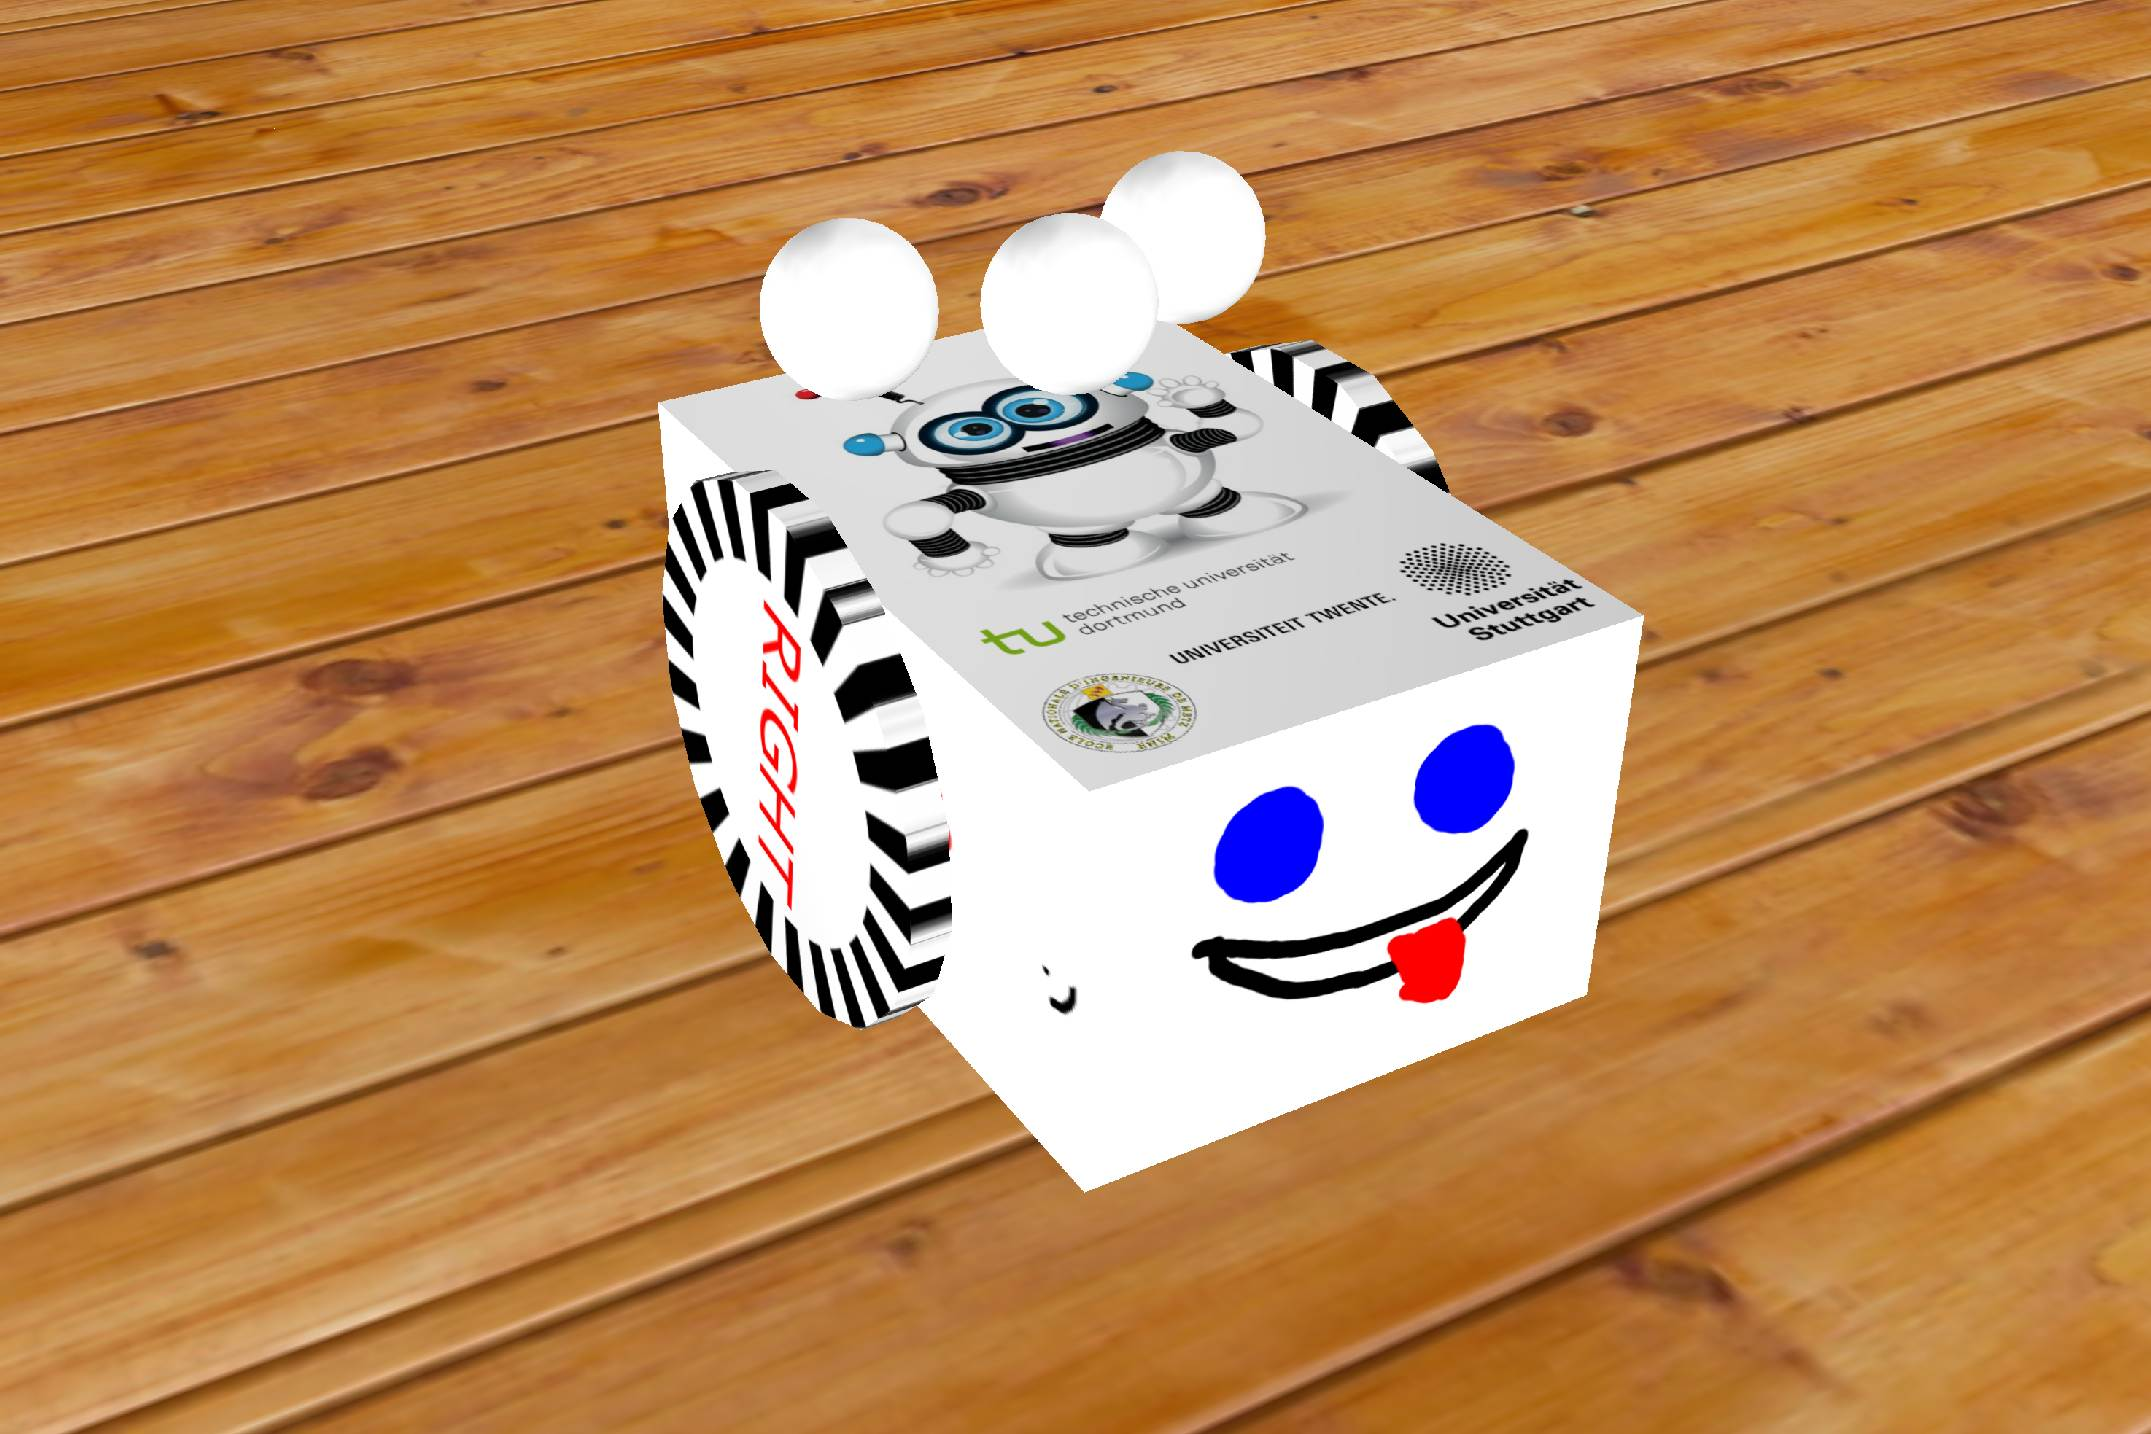
\includegraphics[width=\picsize]{summerSchoolModels/Group3robot}
} \\
\subfigure[Group 4]{\label{fig:group4}
  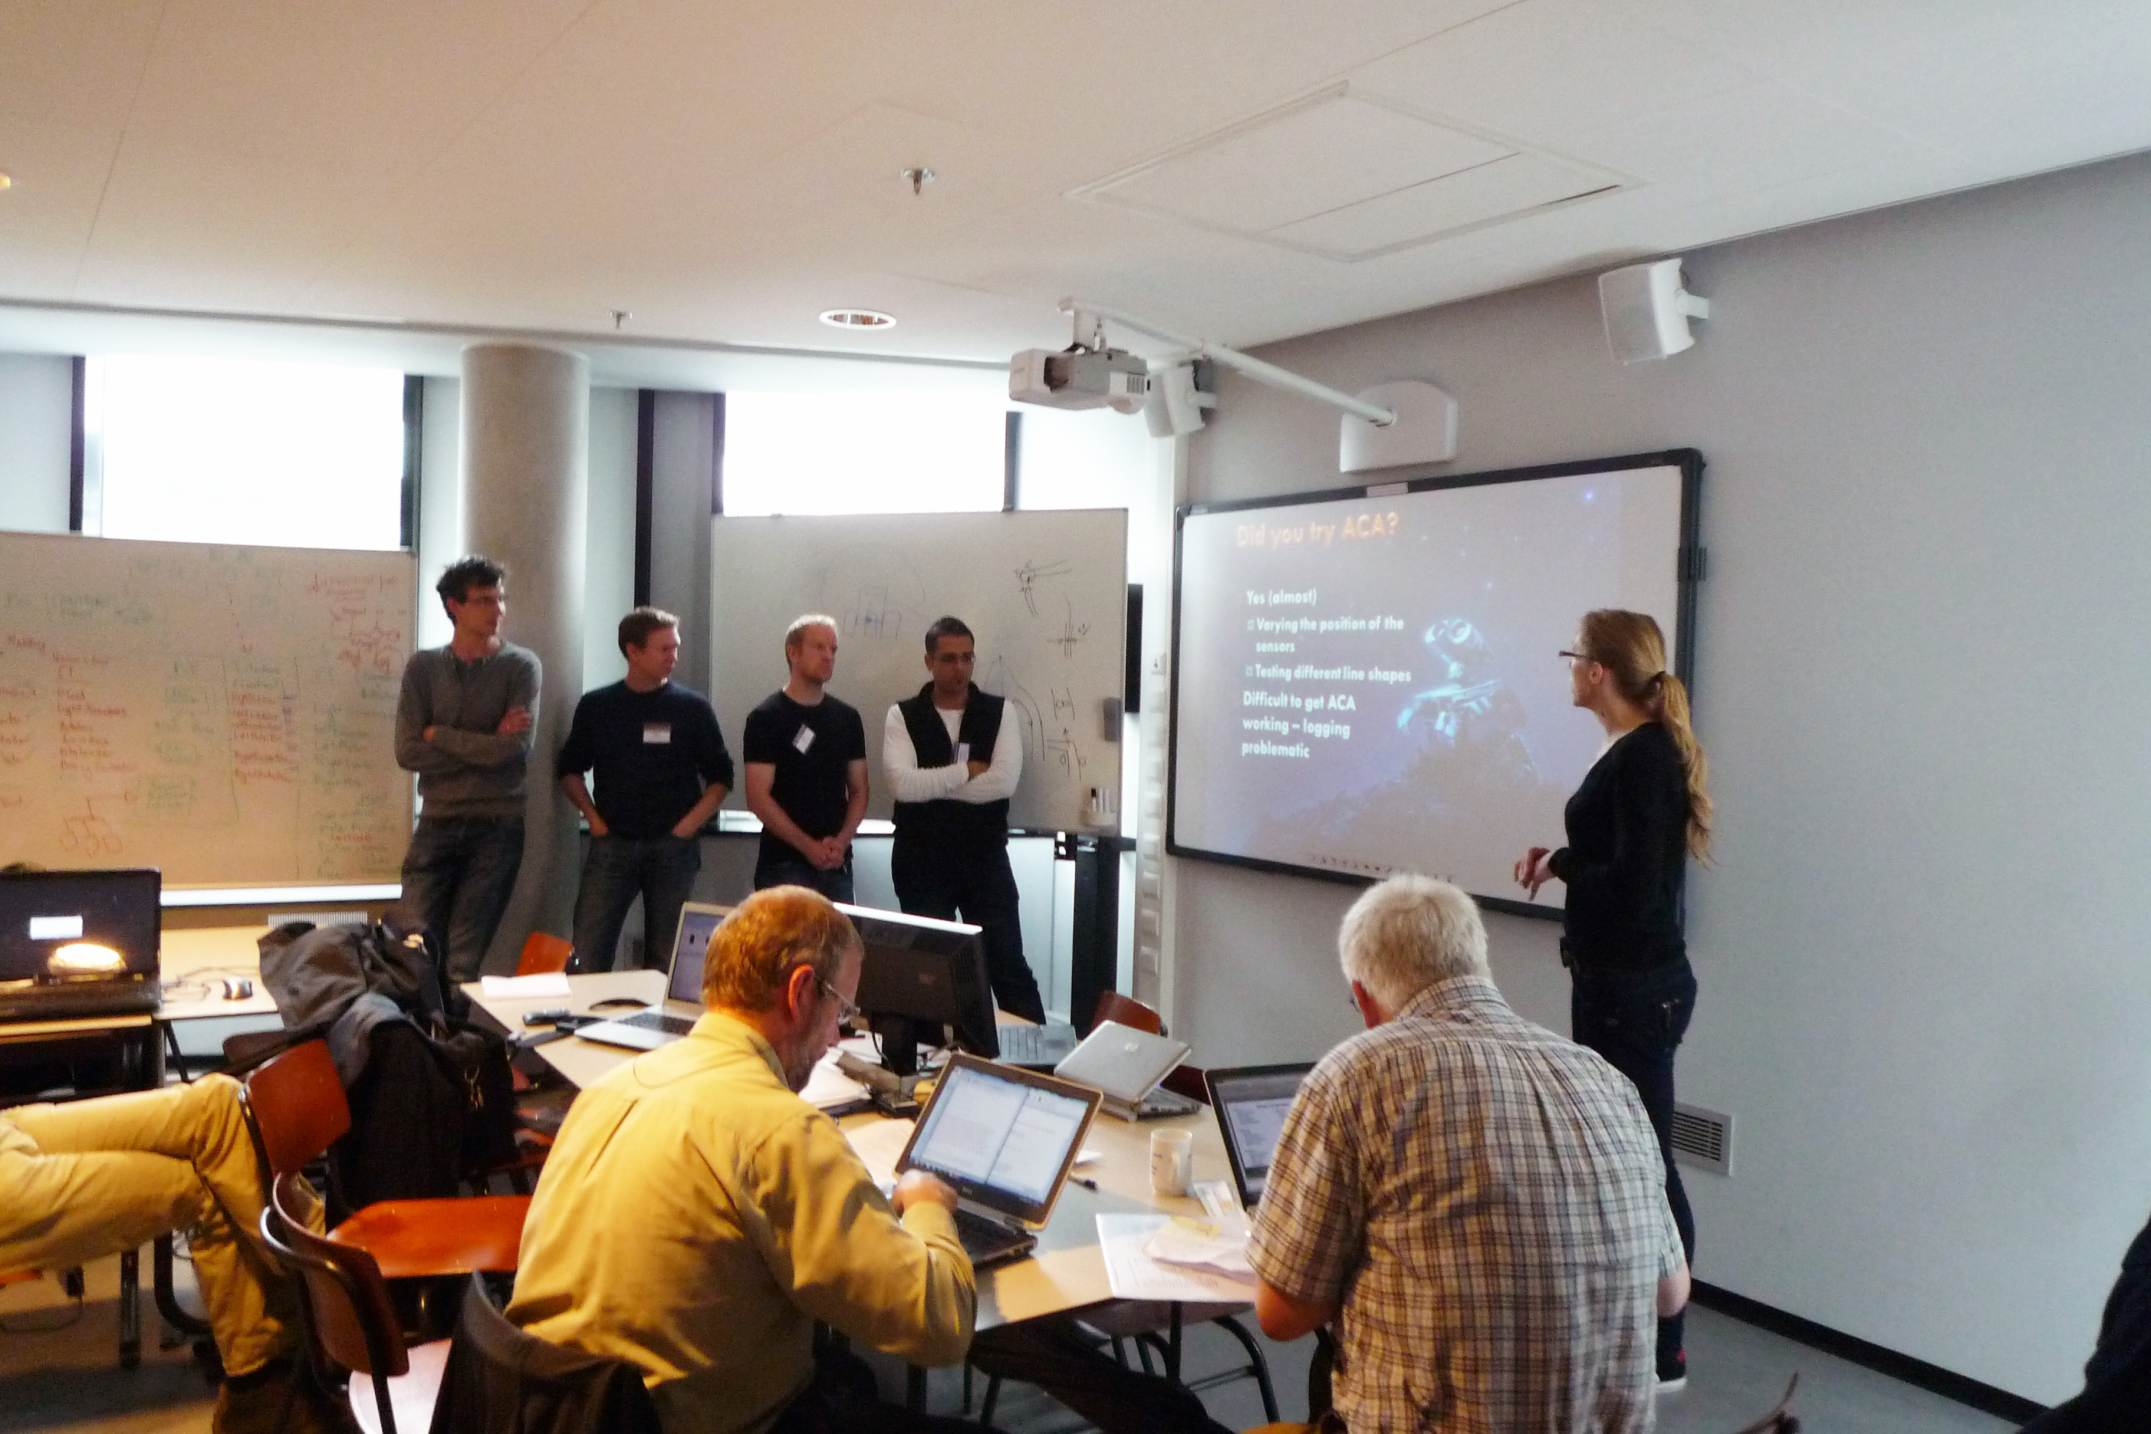
\includegraphics[width=\picsize]{summerSchoolModels/Group4} \quad
  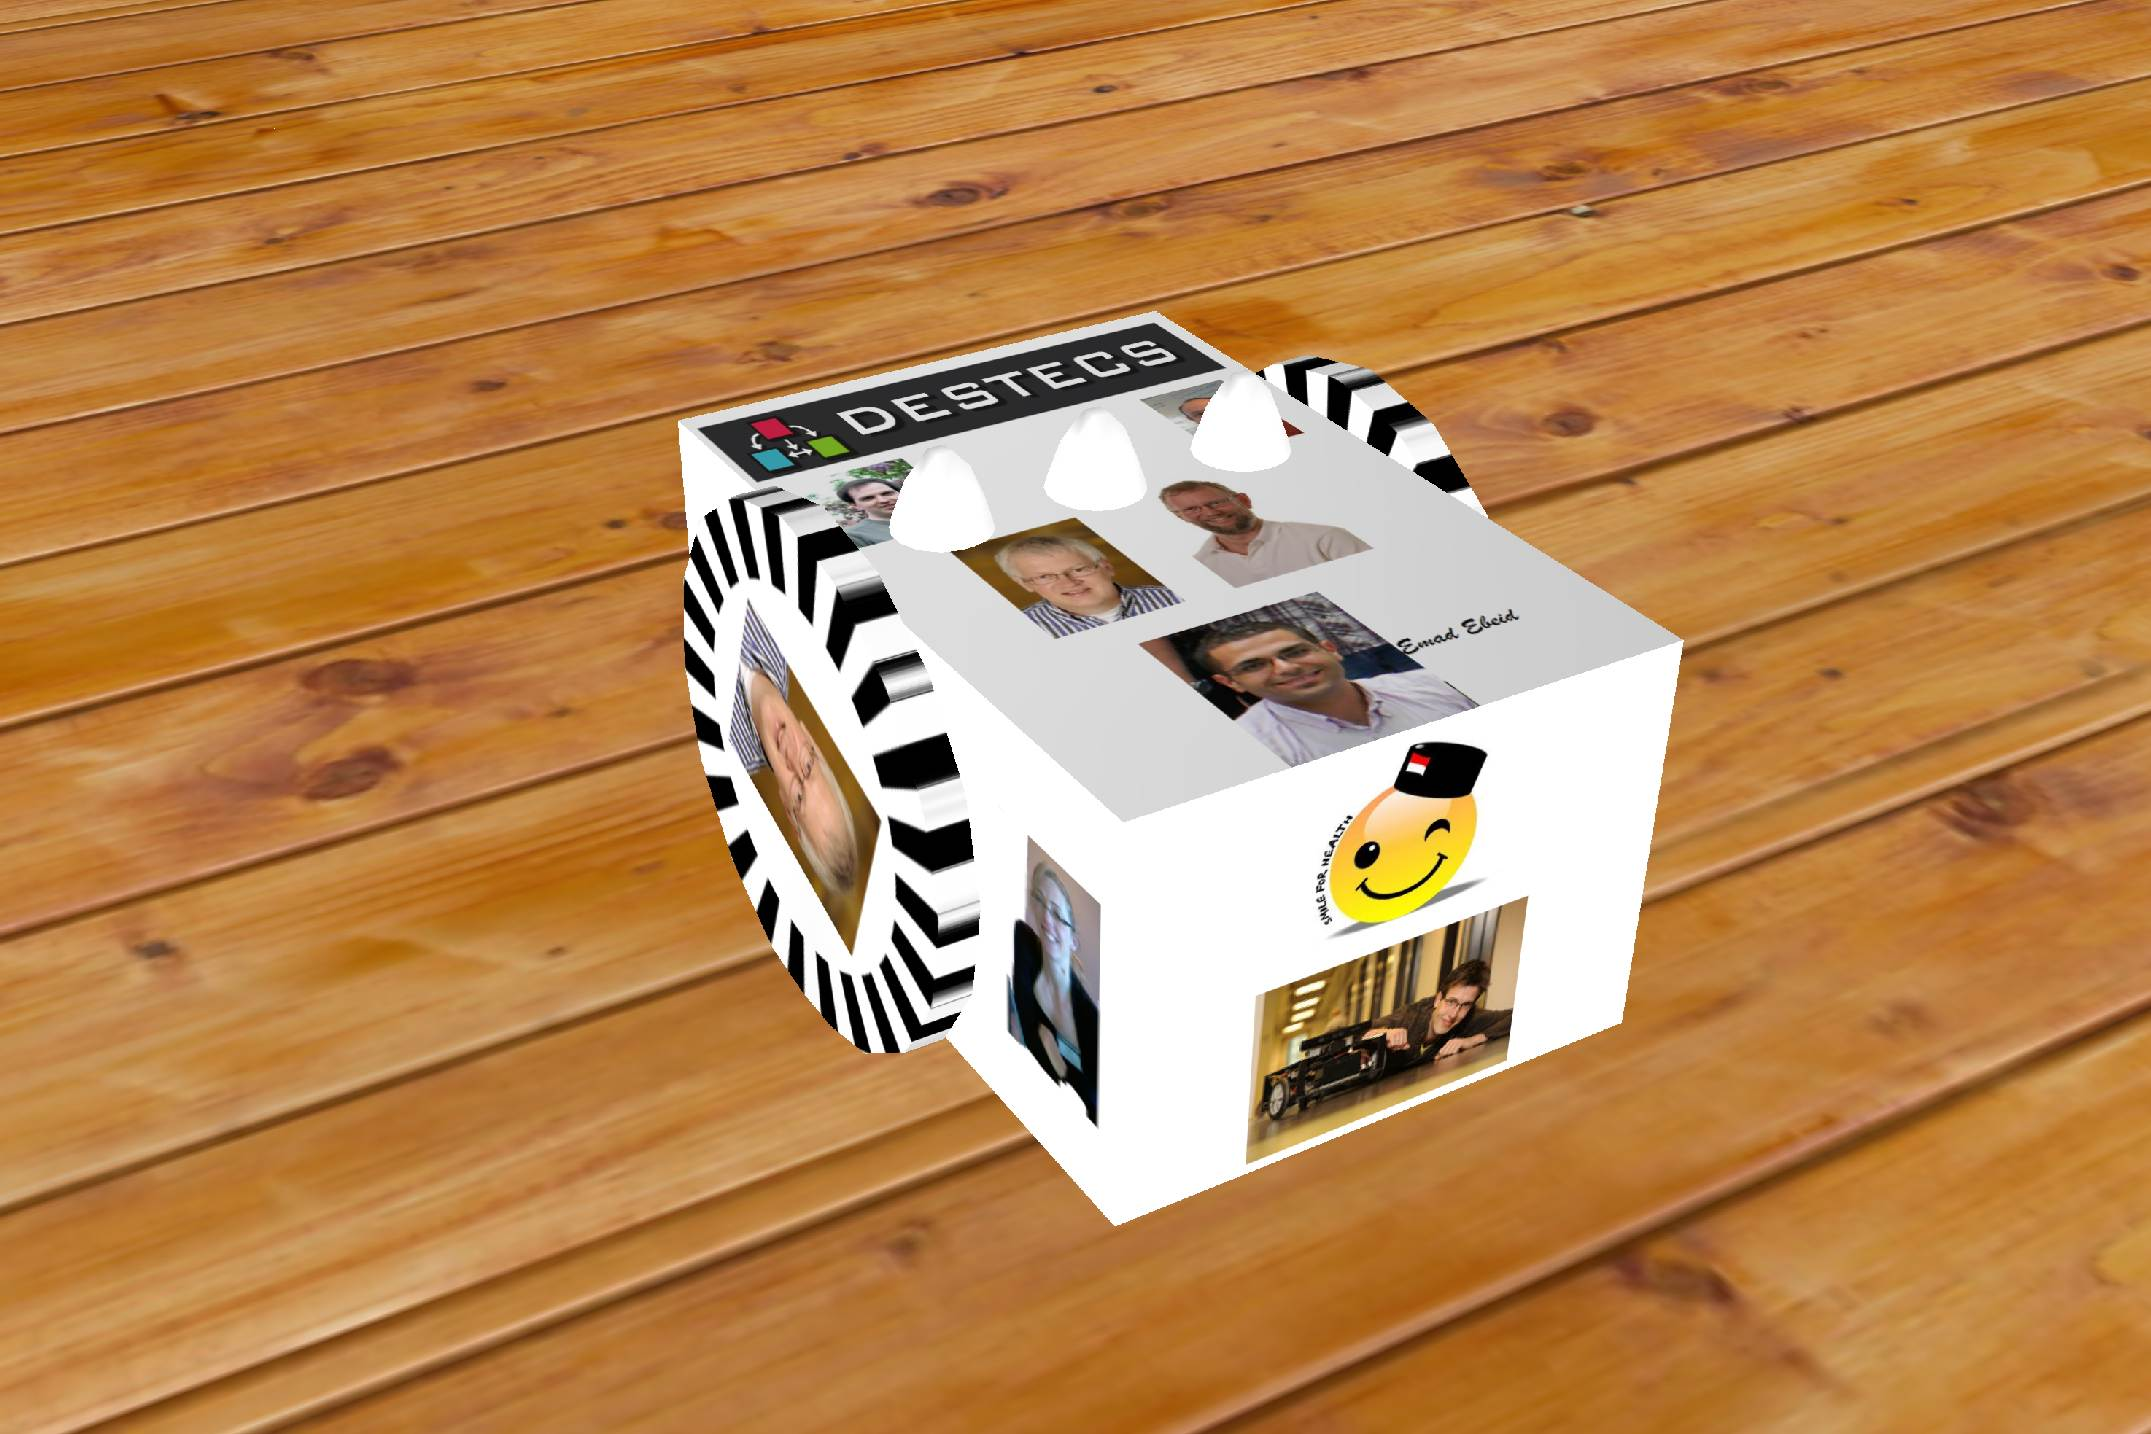
\includegraphics[width=\picsize]{summerSchoolModels/Group4robot}
} \\
\subfigure[Group 5]{\label{fig:group5}
  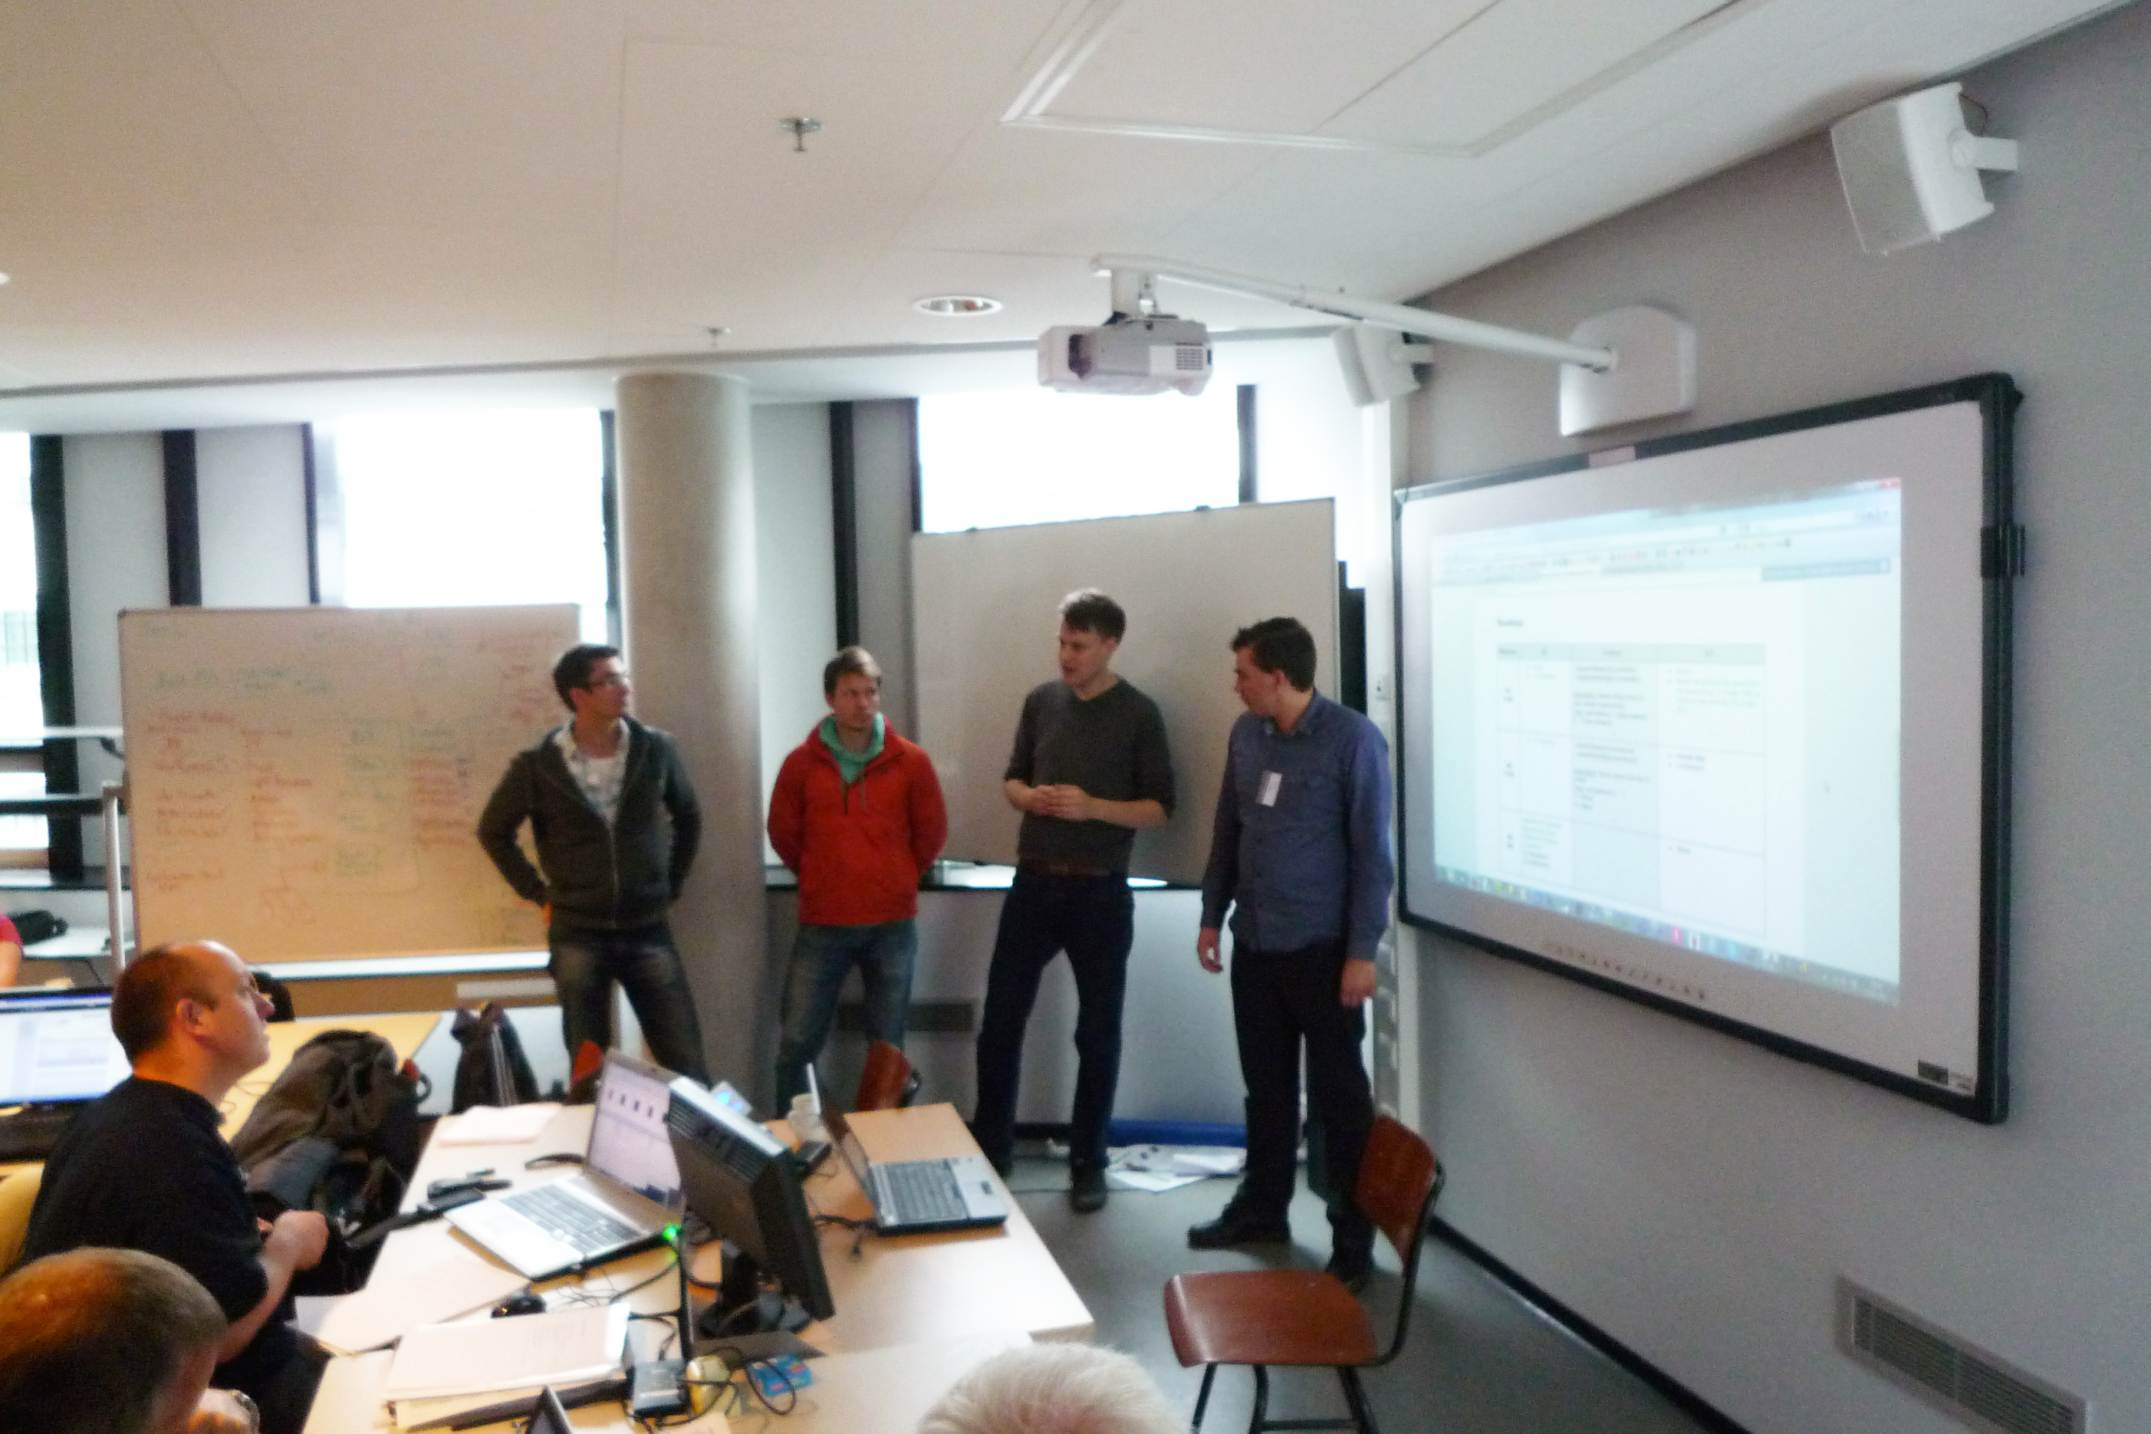
\includegraphics[width=\picsize]{summerSchoolModels/Group5} \quad
  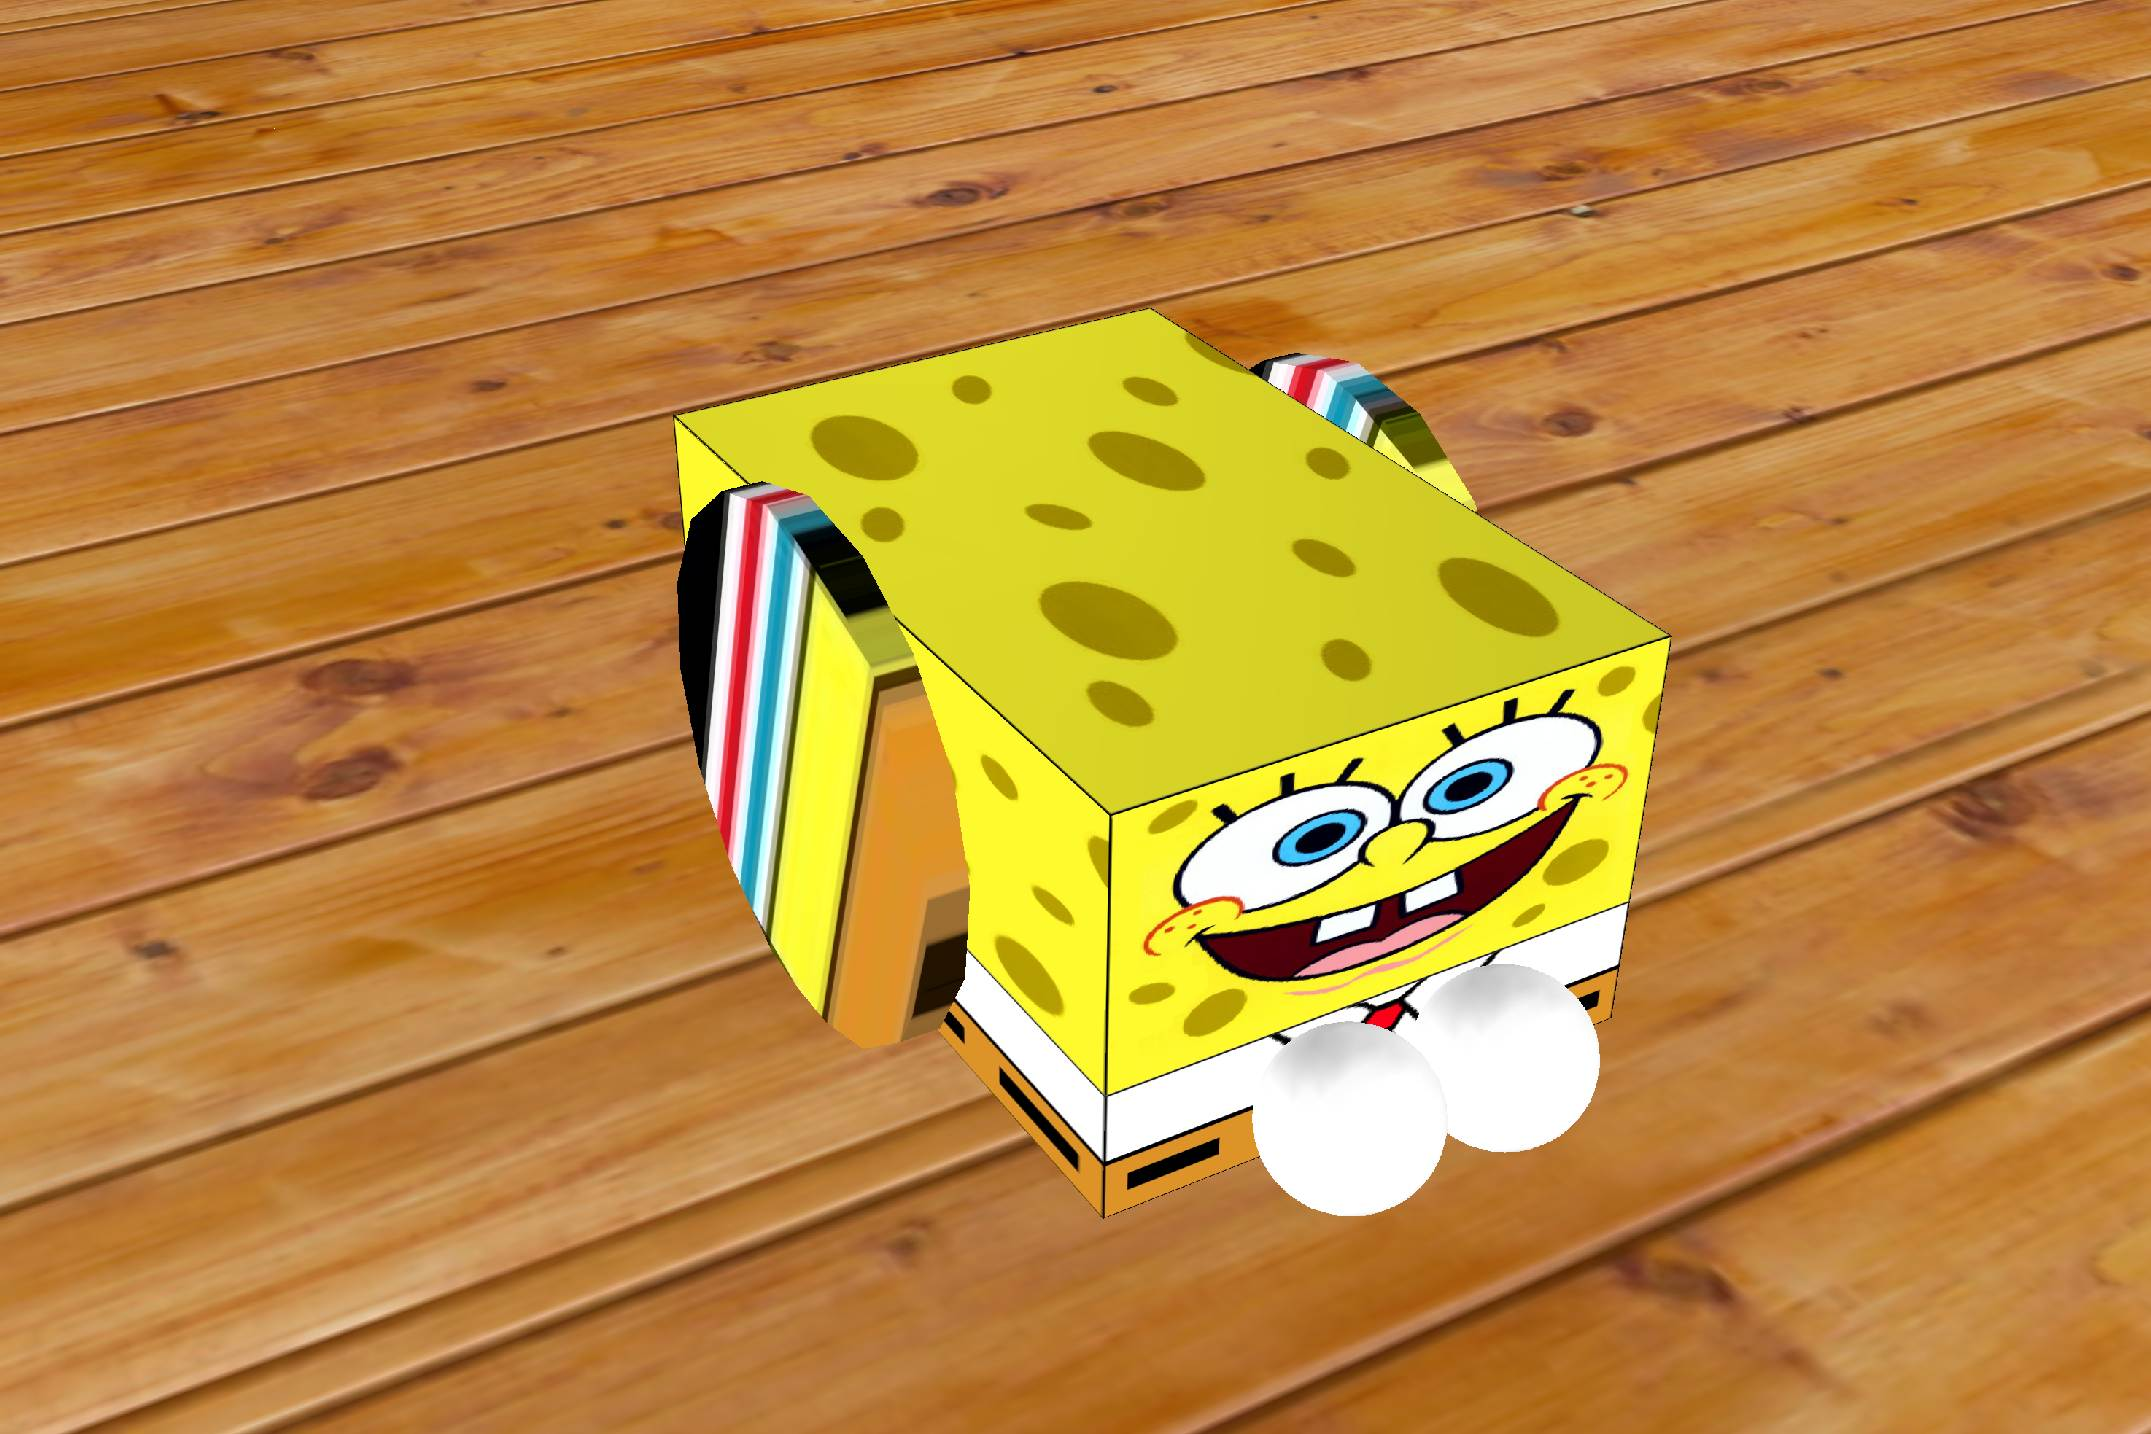
\includegraphics[width=\picsize]{summerSchoolModels/Group5robot}
}
\caption{Photograph of each group and a screenshot of their robot design}
\label{fig:groupphotos}
\end{figure}

